\providecommand{\main}{../../../..}
\documentclass[\main/dresen_thesis.tex]{subfiles}
  \renewcommand{\thisPath}{\main/chapters/monolayers/structureModel/verticalStructure}

\begin{document}
  As discussed in \refch{sec:theoreticalBackground:scattering:reflectometry}, reflectometry is an excellent method to resolve the vertical structure of a sample.
  X-ray reflectometry yields information on the average electron density distribution with respect to the vertical axis, whereas neutron reflectometry yields information on the nuclear structure and in case of polarized neutrons additionally on the spin density.

  Parrats recursive method is most efficient for samples that have in average a constant lateral scattering length density (SLD) for relative large parts of their height, as it models the density profile using slabs and interfacial roughness as parameters.
  This is beneficial for the case of nanocubes in a square lattice, as they can be described by very few parameters.

  \begin{figure}[tb]
    \centering
    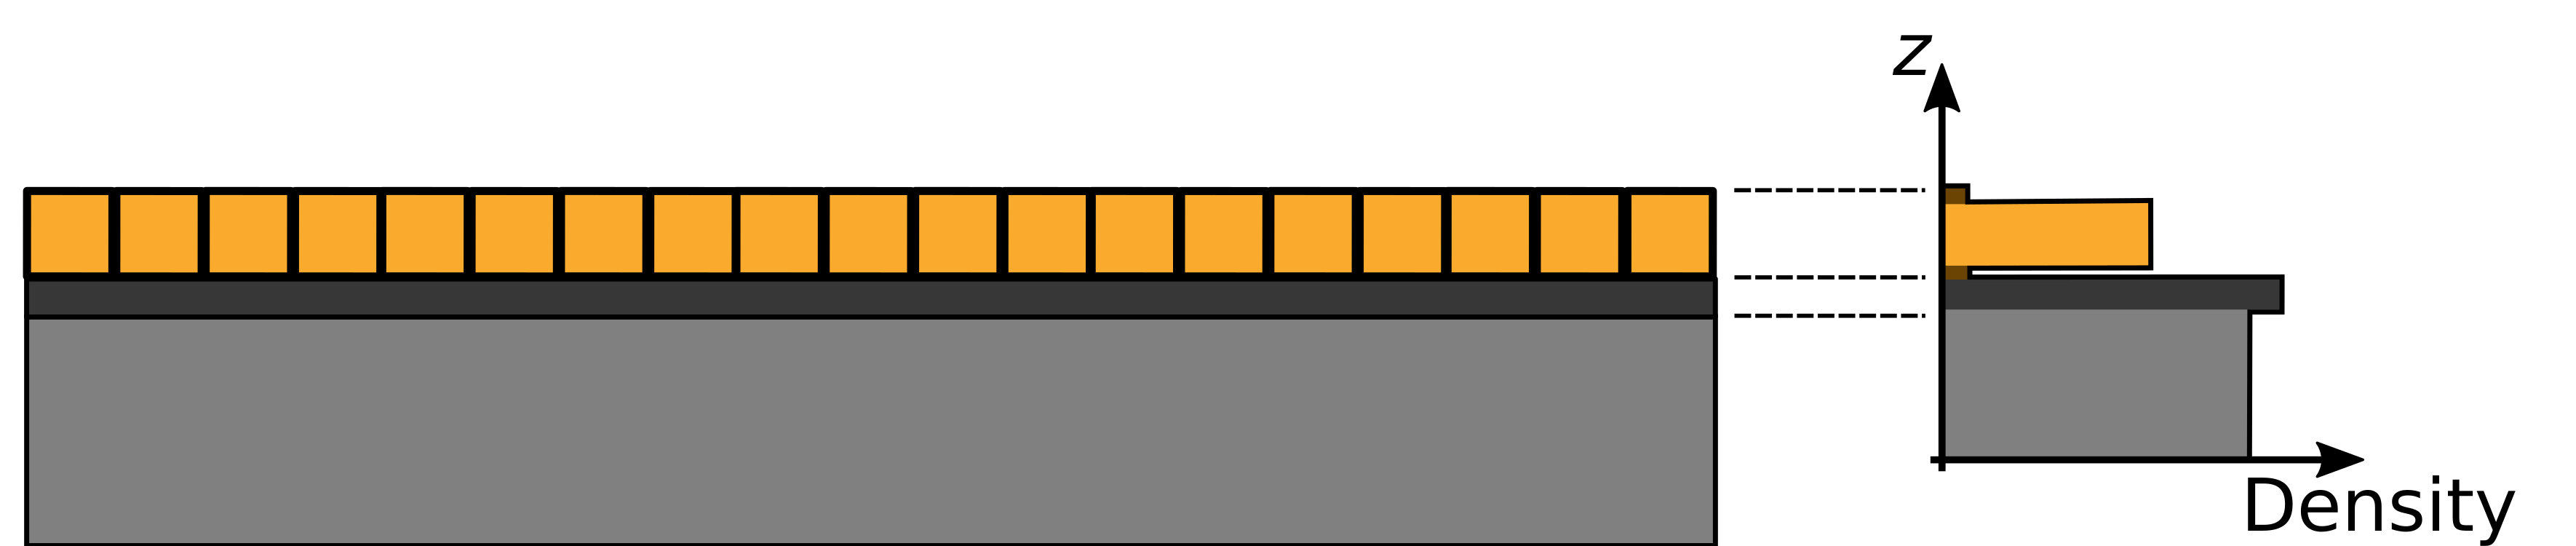
\includegraphics{monolayers_structure_verticalModel}
    \caption{\label{fig:monolayers:structure:verticalModel}Model for a square array of nanocubes depicted as cartoon of the cross-section (left) and the expected resulted shape of the vertical density structure (right).}
  \end{figure}

  The model that is used in this section to discuss reflectometry data is depicted schematically in \reffig{fig:monolayers:structure:verticalModel}.
  The lower gray area represents the silicon substrate with the possibility of a silicion dioxide (\ch{SiO2}) or another organic residue layer in between substrate and nanocubes.
  The average lateral density of a square array layer is modeled by a single slab, with lower density slabs for possible oleic acid spacers (OA) around it.
  Due to the different surroundings for both OA layer (silicon/OA/particle, particle/OA/air), the density and thickness of each is allowed to vary independently.
  And at last, which is not depicted in \reffig{fig:monolayers:structure:verticalModel}, the interfaces are not clear cuts in the vertical plane but have a certain interfacial roughness, which are treated by roughness parameters in the model for each type of interface.

  In total the ideal model has $8$ structural parameters: $4$ parameters to describe the thickness of the nanocubes, the two OA and the \ch{SiO2} layers and $4$ roughness parameters for the interfaces \ch{Si}/\ch{SiO2}, \ch{SiO2}/OA, OA/nanocube and OA/air.
  Additionally it has $5$ parameters to describe the SLD of the nanocubes, the two OA, the \ch{SiO2} and the substrate layer.
  By complementary experiments the number of parameters can be reduced a little.
  The edge length of the nanocubes is already determined by the small-angle scattering experiments and can be fixed in the model.
  As also SLD is determined by SAS, the parameter can be translated to a packing density of the nanocubes in reflectometry.
  Furthermore, the substrate properties and the check for a \ch{SiO2} layer is measured from an empty wafer, which in theory further determines the SLD of \ch{Si}, the \ch{SiO2} thickness and SLD and the \ch{Si}/\ch{SiO2} roughness.
  Additional to the described model property parameters, instrumental parameters are included in the model: the instrumentalresolution needs to be considered either by including angular divergence and energy resolution or by using the resolution function that is known from the instrument.
  Also as the sample alignment has finite precision, a small linear shift in $q$ is allowed in the model.

  The x-ray reflectometry data has been measured at ambient conditions on an Bruker D8 instrument at the \textsc{Forschungszentrum J\"ulich}, which is described in \refapp{app:additionalExperimentalTechniques:xrr}.
  After definition of the model and its parameters, the parameter values are refined by applying the Levenberg-Marquardt algorithm \cite{Marquardt_1963_Analgo}, to minimize the figure of merit $\mathrm{FOM}$, which is defined here for reflectometry as
  \begin{align}
    \mathrm{FOM} \eq \sum_{q_i} \biggl( \frac{\log(I) - \log(I_\mathrm{model})}{\sigma_{I}} I\biggr)^2.
  \end{align}
  The definition is analogue to the $\chi^2$ function, but on the logarithmic scale to avoid that the algorithm only fits the high intensity region at small $q$.

  \begin{figure}[tb]
    \centering
    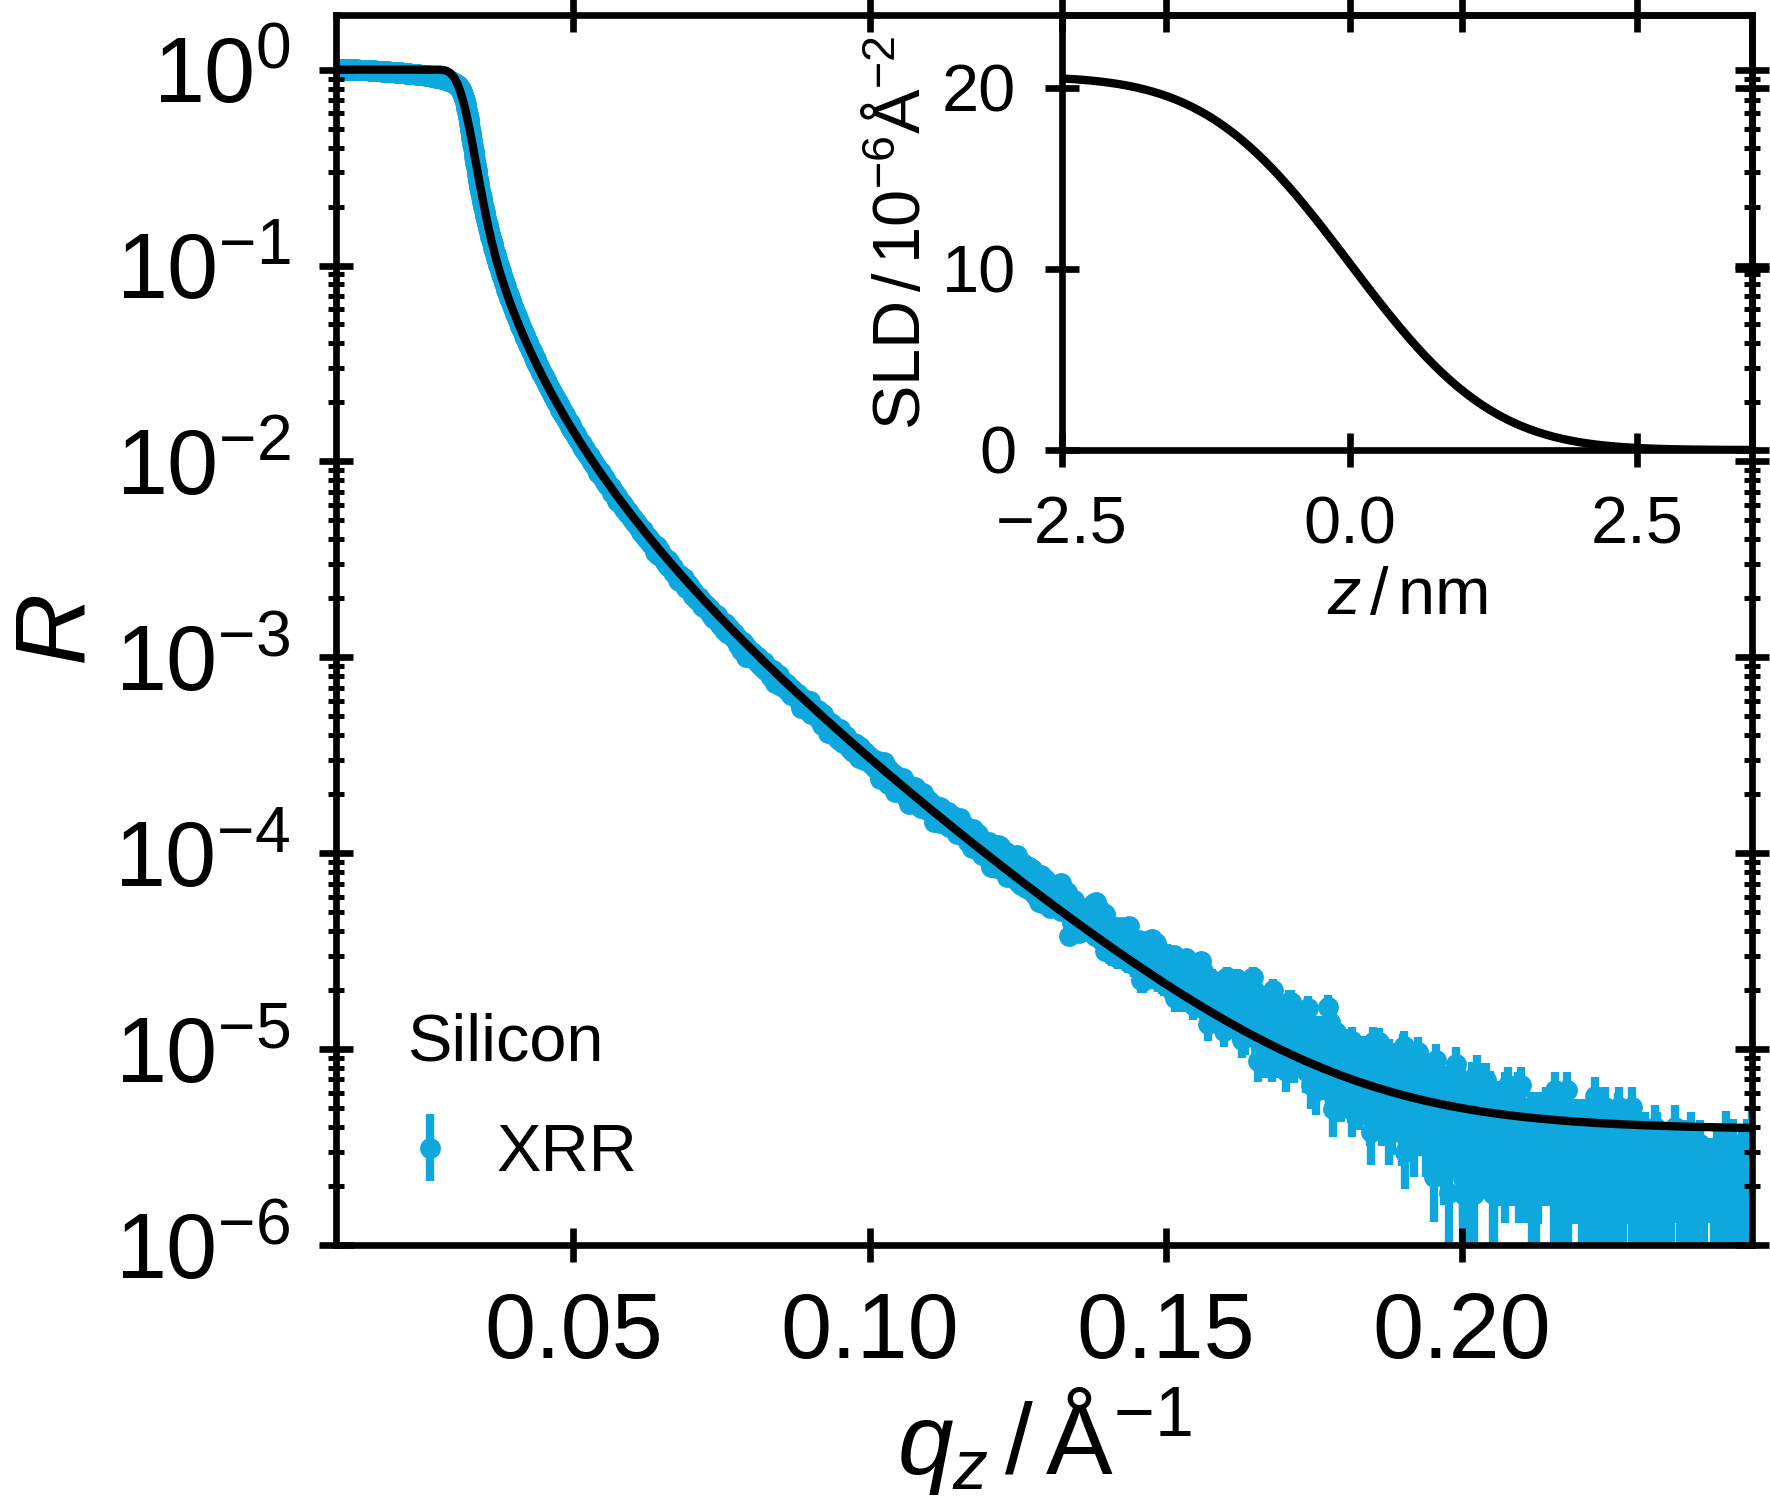
\includegraphics{monolayers_VerticalStructure_SiliconSubstrate_XRR}
    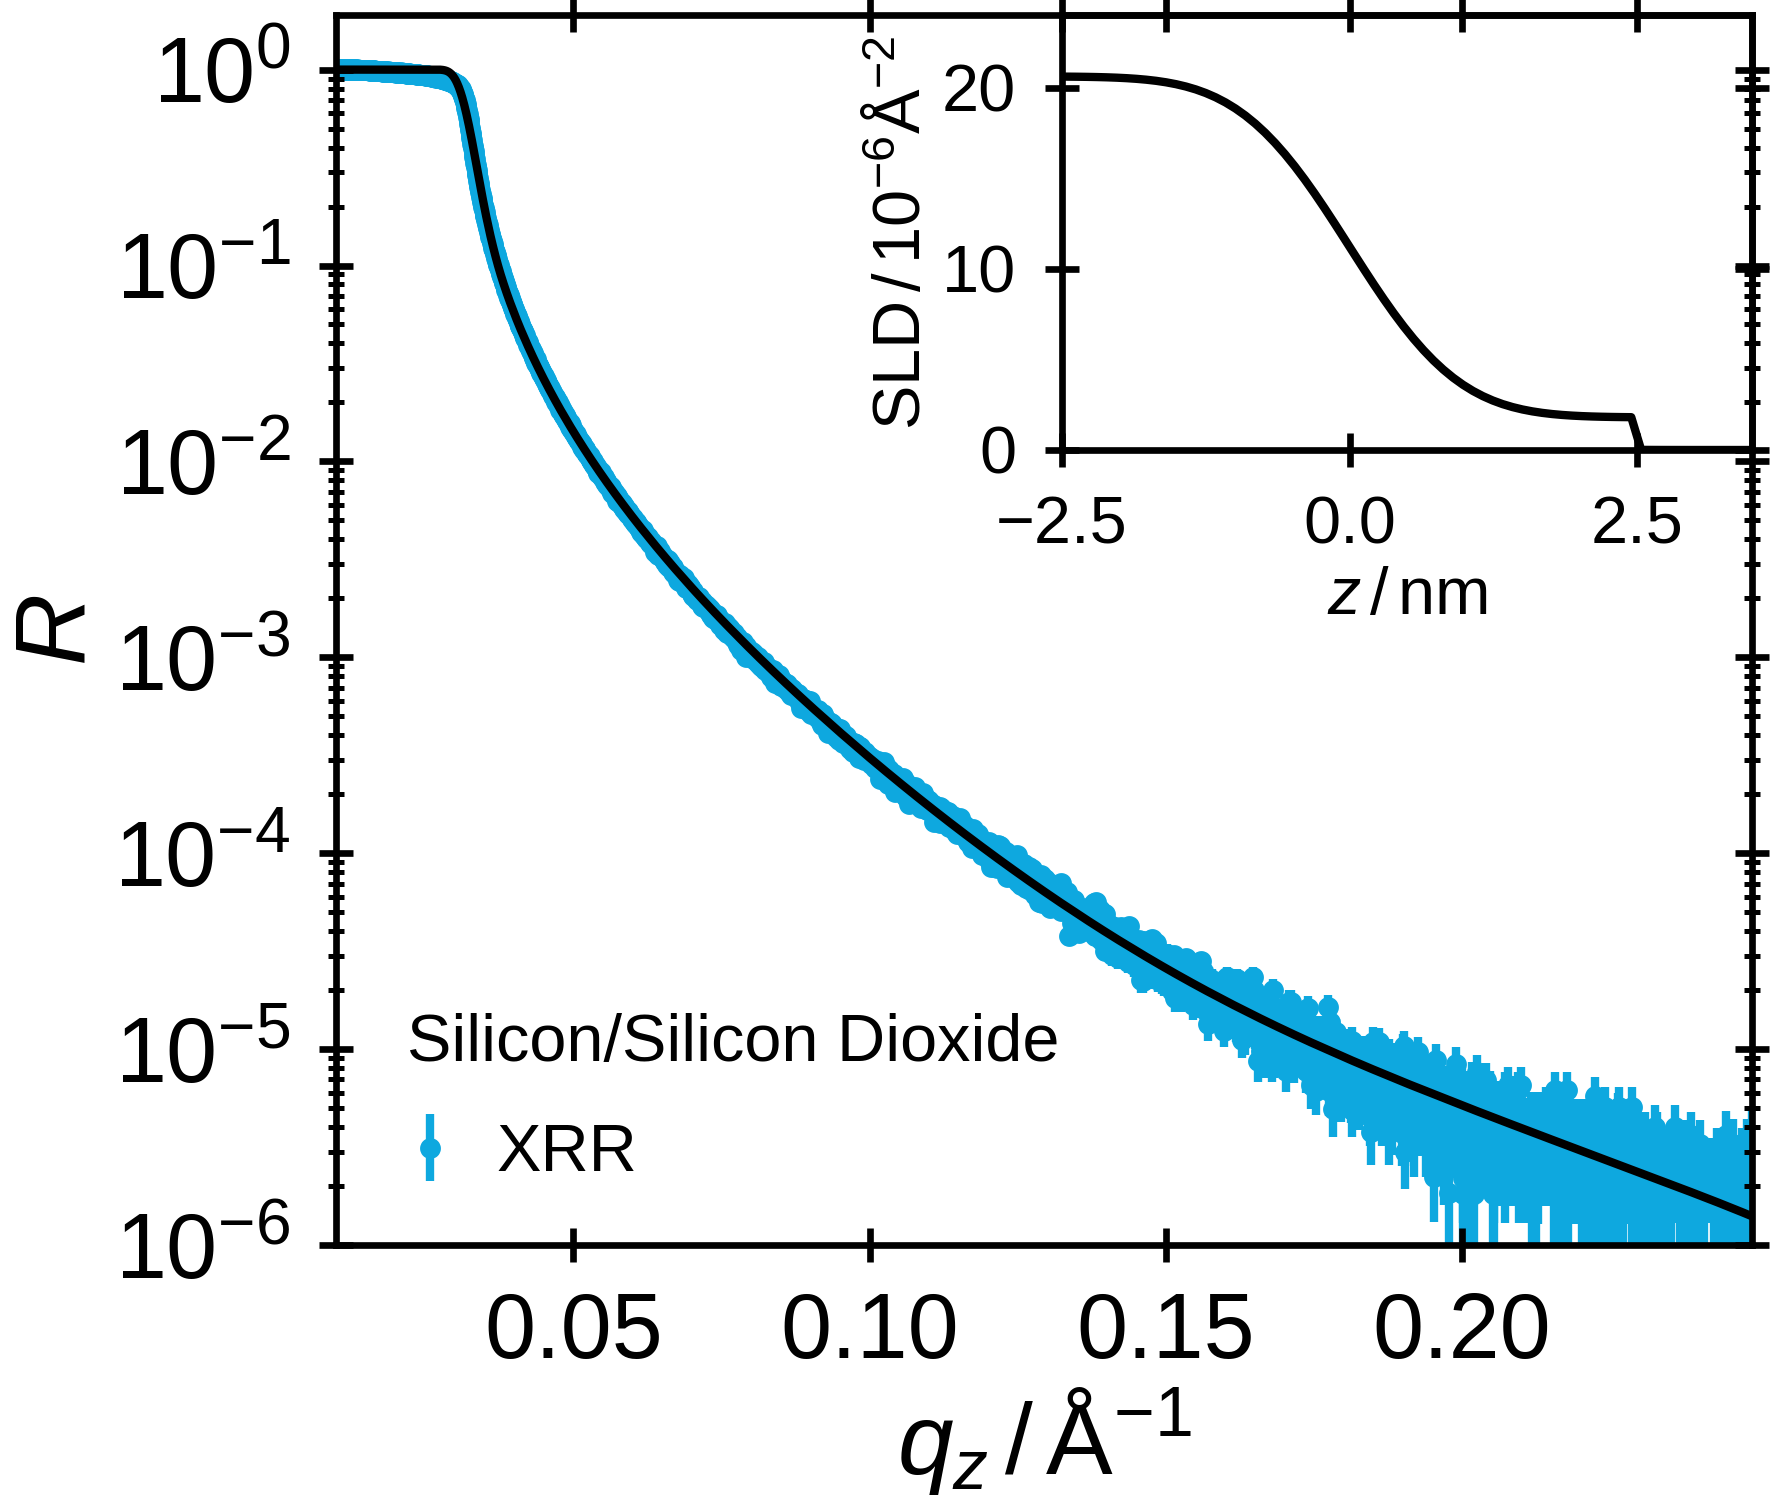
\includegraphics{monolayers_VerticalStructure_SiliconSiliconDioxide_XRR}
    \caption{\label{fig:monolayers:structure:emptySiliconWafer}Empty silicon substrate charachterized by XRR using a bare substrate model (left) and a single layer model (right).}
  \end{figure}
  \begin{table}[ht]
    \centering
    \caption{\label{tab:monolayers:structure:emptySiliconWafer}Parameter values for the model used to describe the x-ray reflectometry of an empty wafer, shown in \reffig{fig:monolayers:structure:emptySiliconWafer}.}
    \begin{tabular}{l | l | l}
      \hline
      &
      Substrate Model &
      Single Layer Model\\
      \hline
      $\sigma_\mathrm{Si}$ &
        $0.982(7)\unit{nm}$ &
        $0.759(7)\unit{nm}$ \\
      $\sigma_{\ch{SiO2}}$ &
        &
        $0.0(0)\unit{nm}$ \\
      $\mathrm{SLD}_{\ch{SiO2}}$ &
        &
        $18.2(6) \cdot \unit{10^{-6} \angstrom^{-2}}$ \\
      $d_{\ch{SiO2}}$ &
        &
        $2.50(5) \unit{nm}$ \\
      \hline
      $\Delta \lambda / \lambda$ &
        $5.24(4) \%$ &
        $5.27(4) \%$ \\
      $q_\mathrm{shift} \,/\, \angstrom^{-1}$ &
        $-7.60(8) \cdot \unit{10^{-4} \angstrom^{-1}}$ &
        $-7.39(7) \cdot \unit{10^{-4} \angstrom^{-1}}$ \\
      $I_\mathrm{bg}$ &
        $3.9(5) \cdot 10^{-6}$ &
        $0.3(4) \cdot 10^{-6}$ \\
      \hline
      $\mathrm{SLD}_{\ch{Si}}$ &
        \multicolumn{2}{c}{$20.061 \cdot \unit{10^{-6} \angstrom^{-2}}$} \\
      $\lambda$ &
        \multicolumn{2}{c}{$1.5418 \unit{\angstrom}$} \\
      \hline
      $\mathrm{FOM}$ &
        $127$ &
        $126$ \\
      \hline
    \end{tabular}
  \end{table}
  The empty wafer XRR, shown in \reffig{fig:monolayers:structure:emptySiliconWafer}, is already very well described by a simple model of only a silicon substrate (left) with surface roughness, background and instrumental resolution as parameters as listed in the left column of \reftab{tab:monolayers:structure:emptySiliconWafer}.
  Adding another slab, to allow for a silicon dioxide layer has shown no significant improvement of the figure of merit.
  However, closer inspection of the model and data on the right of \reffig{fig:monolayers:structure:emptySiliconWafer}, shows  with the additional layer, the low intensity data at high $q$ are described more naturally within the model and without the need of an instrumental background parameter.
  Within both models, the SLD of the silicon substrate was taken from the literature value of silicon that is determined for a density of $\rho_{\ch{Si}} \eq 2.329 \unit{g \, mL^{-1}}$ \cite{Lide_2004_Handb}.
  The SLD obtained for the second layer is significantly below that of \ch{SiO2} ($\mathrm{SLD}_{\ch{SiO2}}^\mathrm{x-ray, \,Lit.} \eq 22.724 \unit{10^{-6} \angstrom^{-2}}$).
  This might hint to a highly porous layer or that the additional layer is not actually \ch{SiO2}.
  As the confidence in the obtained properties of the surface layer are vague, the parameters are kept variable in the model fitting process of the monolayer.

  \begin{figure}[tb]
    \centering
    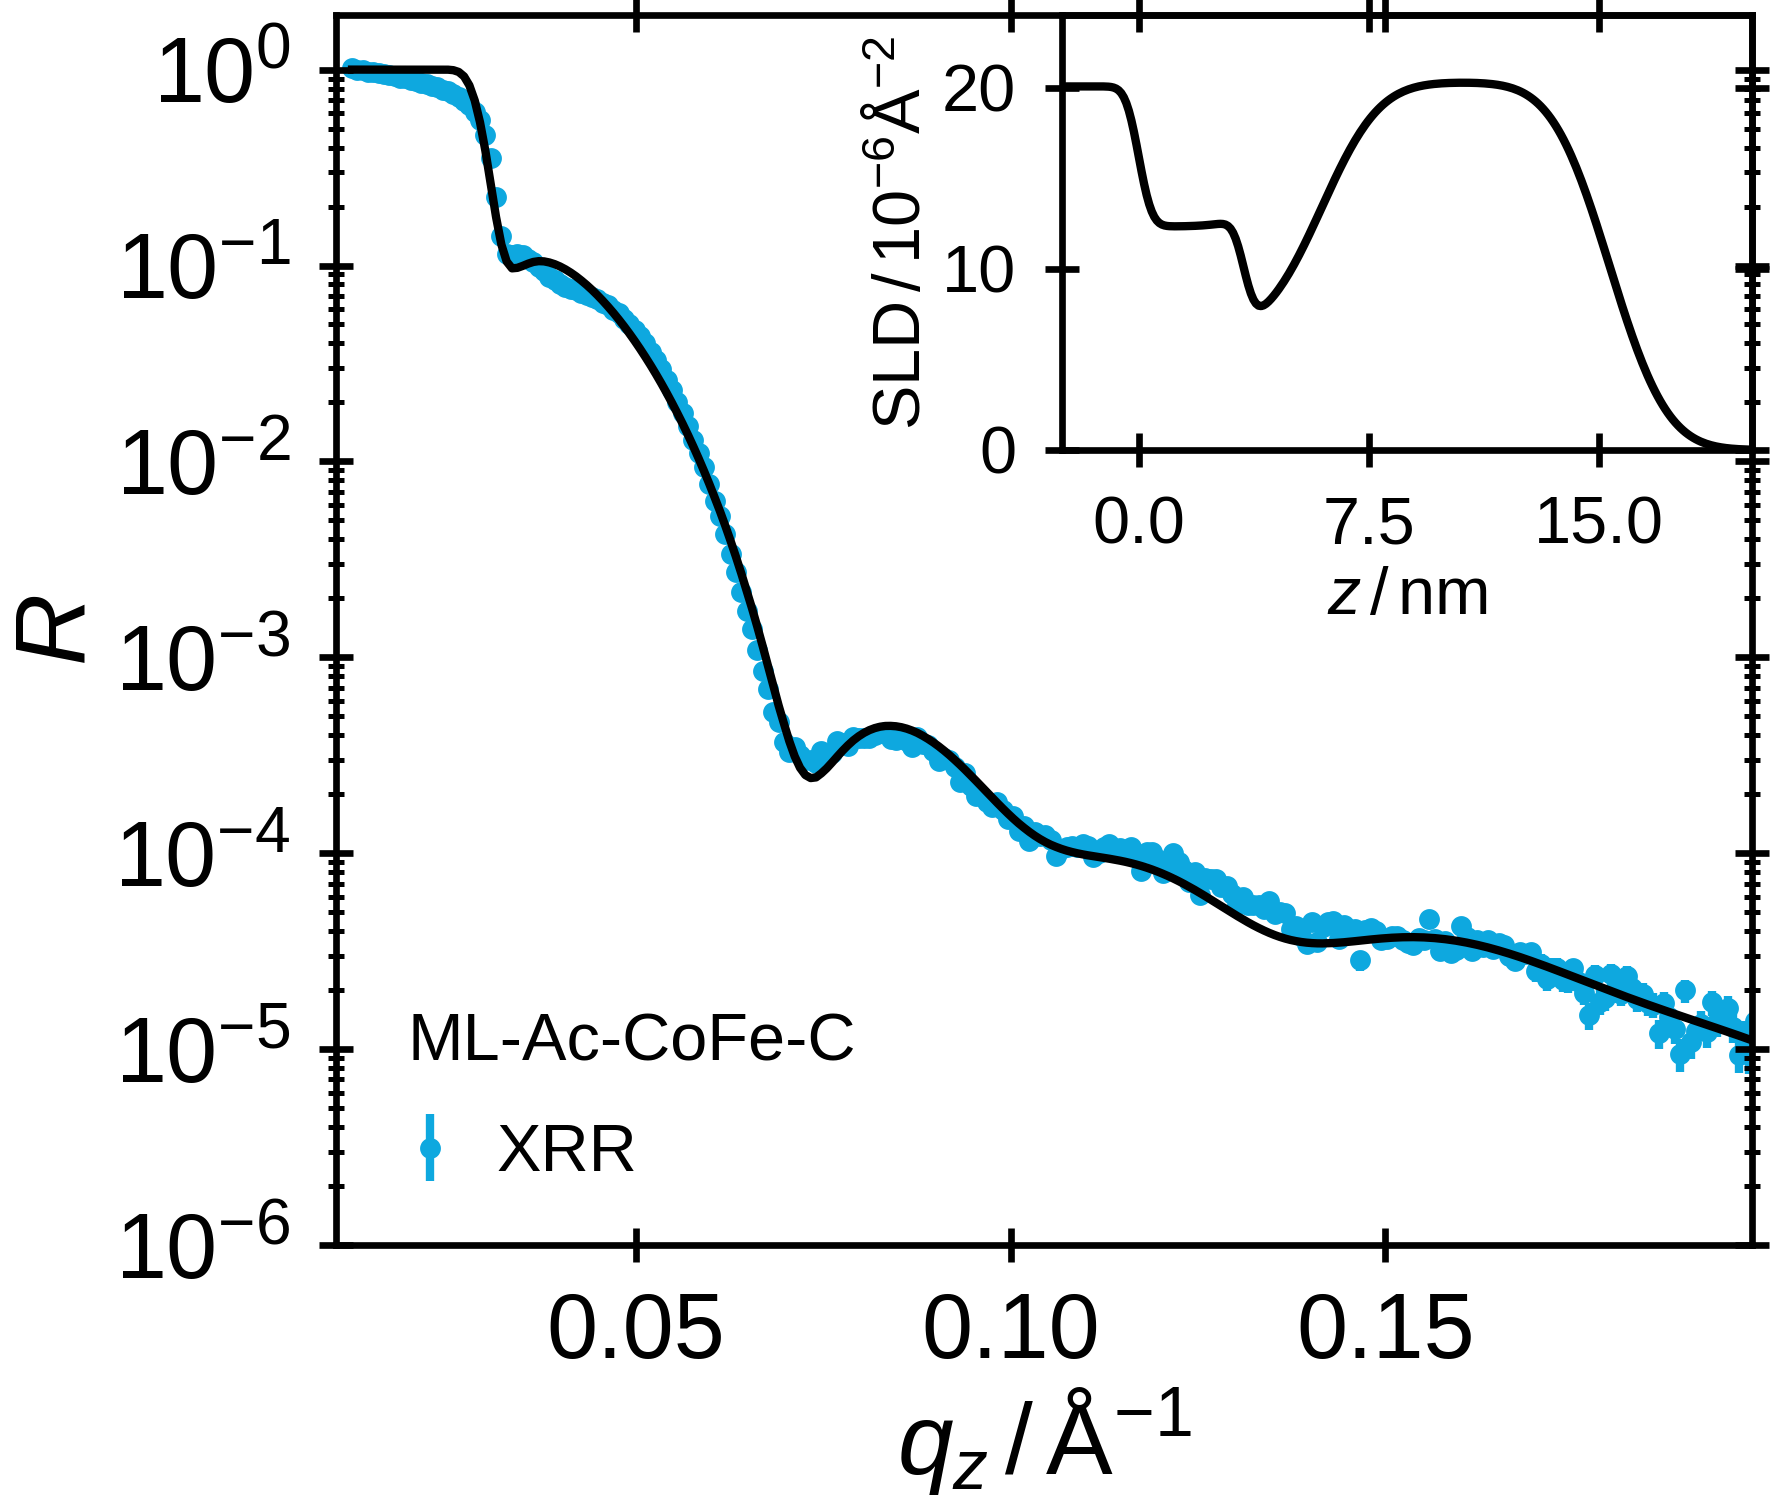
\includegraphics{monolayers_VerticalStructure_ML_Ac-CoFe-C_WithSpacer_XRR}
    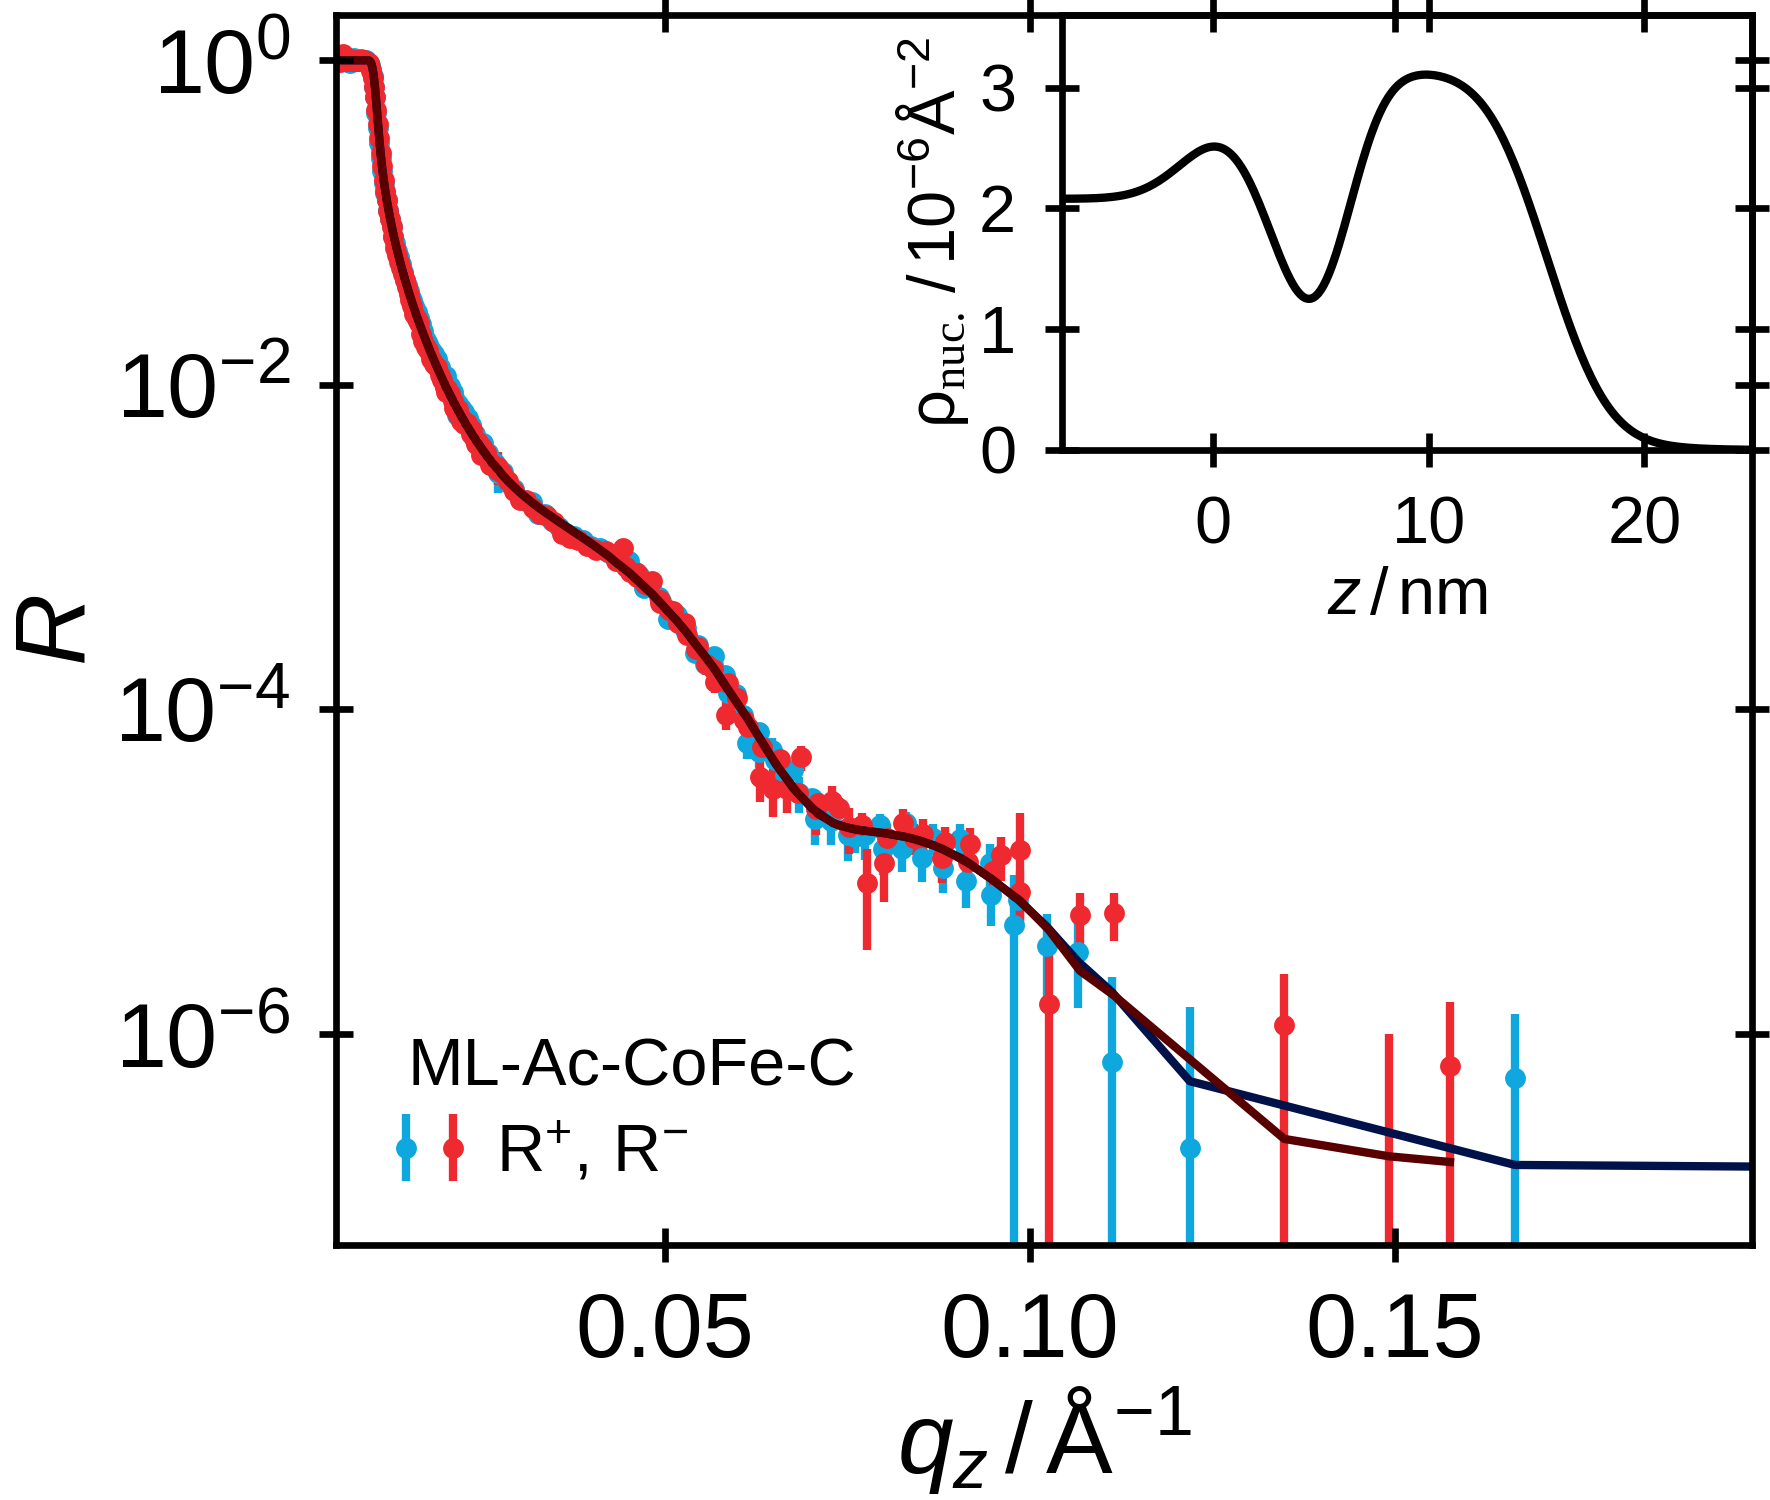
\includegraphics{monolayers_VerticalStructure_ML_Ac-CoFe-C_WithSpacer_NR}
    \caption{\label{fig:monolayers:structure:XRR:ML-Ac-CoFe-C-WithSpacer}X-Ray (left) and neutron
    reflectometry of ML-Ac-CoFe-C described by the model presented in \reffig{fig:monolayers:structure:verticalModel} with the same structural parameters in both cases.}
  \end{figure}


  \begin{table}[ht]
    \centering
    \caption{\label{tab:monolayers:structure:ML-Ac-CoFe-C-WithSpacer}Model parameters used to describe x-ray and neutron reflectometry of ML-Ac-CoFe-C used for the description in \reffig{fig:monolayers:structure:XRR:ML-Ac-CoFe-C-WithSpacer}.}
    \begin{tabular}{l | c | c}
      \hline
      &
      XRR &
      NR, 5 K, 10 mT\\
      \hline
      $a \, / \unit{nm}$ &
      \multicolumn{2}{c}{$9.38$} \\
      \hline
      $\eta_\mathrm{Cube} \, /\, \%$ &
        \multicolumn{2}{c}{$48.9(5) $} \\
      $d_{\ch{SiO2}} \, / \unit{nm}$ &
        \multicolumn{2}{c}{$3.6(1)$} \\
      $d_{\mathrm{OA, lower}}$ &
        \multicolumn{2}{c}{$2.35(8)$} \\
      $d_{\mathrm{OA, upper}}$ &
        \multicolumn{2}{c}{$0.00$} \\
      $\sigma_{\ch{Si}/\ch{SiO2}} \, / \unit{nm}$ &
        \multicolumn{2}{c}{$0.23(5)$} \\
      $\sigma_{\ch{SiO2}/\mathrm{OA}}\, / \unit{nm}$ &
        \multicolumn{2}{c}{$0.3(7)$} \\
      $\sigma_\mathrm{OA/Cube} \, / \unit{nm}$ &
        \multicolumn{2}{c}{$1.22(6)$} \\
      $\mathrm{SLD}_\mathrm{Cube} \, / \unit{10^{-6} \angstrom^{-2}}$ &
        $41.749$ &
        $6.09(2)$ \\
      $\mathrm{SLD}_{\ch{SiO2}} \, / \unit{10^{-6} \angstrom^{-2}}$ &
        $12.1(3)$ &
        $2.26$ \\
      $\mathrm{SLD}_\mathrm{OA} \, / \unit{10^{-6} \angstrom^{-2}}$ &
        $6.5(5)$ &
        $0.58(2)$ \\
      \hline
      $\mathrm{SLD}_{\ch{Si}} \, / \unit{10^{-6} \angstrom^{-2}}$ &
        $20.061$ &
        $2.072$ \\
      $\Delta \lambda / \lambda$ &
        $5.25 \%$ &
        from inst. spec.\\
      $q_\mathrm{shift} \,/ \unit{10^{-3} \angstrom^{-1}}$ &
        $-2.571(2)$ &
        $0.0$\\
      $I_\mathrm{bg}$ &
        $0.0 \cdot 10^{-6}$ &
        $0.0 \cdot 10^{-6}$ \\
      $\lambda \, / \unit{\angstrom}$ &
        $1.5418$&
        TOF\\
      \hline
    \end{tabular}
  \end{table}

  \reffig{fig:monolayers:structure:XRR:ML-Ac-CoFe-C-WithSpacer} shows both XRR and NR data measured for ML-Ac-CoFe-C.
  The NR data is measured at the reflectometer D17 at the Institute Laue-Langevin in time-of-flight mode.
  The detailed description of the neutron reflectometer can be found in detail in \refapp{ch:appendix:lss:d17}.
  The shown reflectometry data is measured after zero field cooling at $\mathrm{T} \eq 5 \unit{K}$ with polarized neutrons at a guide field of $B \eq 10 \unit{mT}$.
  Further data taken for ML-Ac-CoFe-C at varied magnetic fields after field and zero-field cooling is discussed in \refsec{sec:monolayers:magneticStructure}.

  To describe both datasets, the model shown in \reffig{fig:monolayers:structure:verticalModel} is first matched with the XRR data and subsequently all structural parameters are fixed for the neutron reflectometry data, while only the scattering length density and instrumental parameters are adjusted.
  The best fit parameters are tabulated in \reftab{tab:monolayers:structure:ML-Ac-CoFe-C-WithSpacer}.
  As the empty silicon wafer showed good agreement with the literature SLD value of silicon, the SLD of the substrate is fixed in both cases and also the energy resolution for the XRR data is fixed to the previously obtained value.
  For the neutron reflectometry data, the resolution from the D17 specification, described in \cite{Gutfreund_2018_Towar}, is used.

  From the obtained packing density, the relative particle spacing $a_{p-p}$ can be estimated by assuming that the measured sample area is approximately a homogeneous square lattice and thus the packing density is given by
  \begin{align}
    \eta \eq \frac{a^2}{a_{p-p}^2}.
  \end{align}
  This results in $a_{p-p} \eq 13.41(7) \unit{nm}$, which is approximately $4 \unit{nm}$ larger than the particle edge length.
  This can reasonably interpreted as a spacing of about two oleic acid chains in between two nanocubes.

  For the $\ch{SiO2}$ layer, the SLD obtained from XRR is scaled to the neutron SLD according to the literature values of the \ch{SiO2} by
  \begin{align}
    \mathrm{SLD}_{\ch{SiO2}}^{\mathrm{neutron} }\eq \frac{\mathrm{SLD}_{\ch{SiO2}}^{\mathrm{neutron, \,Lit.}}}{\mathrm{SLD}_{\ch{SiO2}}^{\mathrm{x-ray, \,Lit.}}} \mathrm{SLD}_{\ch{SiO2}}^{\mathrm{x-ray}},
  \end{align}
  where the literature value for the SLD of $\ch{SiO2}$ for neutrons is given by $\mathrm{SLD}_{\ch{SiO2}}^{\mathrm{neutron, \,Lit.}} \eq 4.186 \cdot \unit{10^{-6} \angstrom^{-2}}$.

  The SLD and thickness of the lower OA layer are slightly off from the literature values $\mathrm{SLD}_{\mathrm{OA}}^{\mathrm{x-ray, \,Lit.}} \eq 8.52 \cdot \unit{10^{-6} \angstrom^{-2}}$ and $\mathrm{SLD}_{\mathrm{OA}}^{\mathrm{neutron, \,Lit.}} \eq 0.078 \cdot \unit{10^{-6} \angstrom^{-2}}$.
  This hints to the possibility that the oleic acid layer is not pure phased but also might contain contaminations.

  In summary, the reflectometry data of both x-ray and neutron reflectometry can be fit by the same model of an homogeneous thin layer structure, thus approving the monolayer property on a large scale.
  The roughness parameters are reasonably small and in case of the nanocube/OA interface comparable to the size distribution of the edge length.
  The determined packing density speaks for a densely packed structure.
  To further quantify the long-ranged in-plane order, grazing-incidence small-angle scattering experiments are discussed and simulated in the following.
\end{document}
